\section{Network Characterization}
\label{sec:analysis}

The analysis is carried out with NetworkX~\cite{networkx} on the simple, undirected and unweighted version of the network, and compared against an Erd\H{o}s--R\'enyi (ER) random graph and a Barab\'asi--Albert (BA) graph with (almost) the same number of nodes and edges. Static plots are produced in Python with Matplotlib, while the community-colored network layout (Figure~\ref{fig:communities}) is produced with Gephi (ForceAtlas2).

\subsection{Degree distribution}
The average degree is $\approx 222$ while the maximum degree reaches $6556$: the distribution is strongly right-skewed, i.e.\ a few hubs coexist with many low-degree accounts. On the log-log CCDF (Figure~\ref{fig:degree}) the empirical curve features a heavy, approximately linear tail, close to the power-law behavior of the BA model and clearly different from the sharply decaying, bell-shaped ER curve. This indicates that the network is approximately scale-free, as expected for a social follow graph dominated by a few highly visible accounts (outlets and prominent communicators).

\begin{figure}[h]
  \centering
  
\includegraphics[width=\linewidth]{figures/degree_ccdf_compare.png}
  \caption{Complementary cumulative degree distribution (CCDF) on a log-log scale: Bluesky vs ER vs BA.}
  \label{fig:degree}
\end{figure}

\subsection{Connected components}
The network has a single connected component covering 100\% of the nodes: the snowball process naturally yields a fully connected network around the seeds, with no isolated nodes. All subsequent path and centrality analyses are therefore performed on the whole graph without loss of nodes.

\subsection{Clustering and density}
The network is sparse in absolute terms (density $0.0148$) yet strongly clustered: the average clustering coefficient is $0.238$ and the global transitivity $0.127$. The empirical clustering, however, is about $16\times$ that of an ER graph of identical density ($0.0148$) and $5\times$ that of a degree-comparable BA graph ($0.0456$), see Table~\ref{tab:compare}. Such a strong tendency toward triangle closure is a clear sign of
community structure and cannot be explained by either random wiring (ER) or pure preferential attachment (BA); it motivates the community detection of Section~\ref{sec:cd}.

\begin{table}[h]
  \centering\small
  \caption{Bluesky vs synthetic graphs (same order of nodes/edges).}
  \label{tab:compare}
  \begin{tabular}{lccc}
    \toprule
    Metric & Bluesky & ER & BA \\
    \midrule
    Nodes             & 15{,}000 & 15{,}000 & 15{,}000 \\
    Edges             & 1{,}665{,}495 & $\approx$1.67M & $\approx$1.67M \\
    Average degree    & 222.1 & 222 & $\approx$222 \\
    Density           & 0.0148 & 0.0148 & 0.0148 \\
    Average clustering & 0.238 & 0.0148 & 0.0456 \\
    Transitivity      & 0.127 & 0.0148 & 0.0465 \\
    Avg. path length$^{*}$  & 2.23 & 2.02 & 2.04 \\
    \bottomrule
  \end{tabular}
\end{table}

{\footnotesize $^{*}$Average path lengths are estimated by sampled BFS (500 sources) on the giant component; the ER value ($2.02$) sits slightly above the leading-order estimate $\ln n / \ln \langle k\rangle \approx 1.8$, which omits lower-order corrections.}


\subsection{Assortativity and mixing}
The degree assortativity coefficient is slightly negative ($-0.07$), so the network is mildly disassortative: high-degree hubs tend to be followed by many low-degree accounts, not by other hubs. This is typical of follow graphs centered on a few highly visible accounts. Mixing by community, in contrast, is strongly positive: the attribute assortativity computed on the Louvain labels is $0.52$, and $59.8\%$ of all edges fall within a single community. Connections are therefore organized far more by topic than by popularity, which quantitatively reinforces the community structure discussed in Section~\ref{sec:cd}.

\subsection{Path analysis}
Estimated on the giant component via sampled BFS, the average shortest-path length is $\approx 2.23$ and the diameter (lower bound) is $\approx 4$. Despite 15{,}000 nodes, any two accounts are on average little more than two hops apart: the network is markedly small-world. The empirical value is only marginally longer than the ER and BA baselines ($2.02$ and $2.04$ under the same sampled-BFS method) and slightly above the leading-order analytical estimate $\ln n / \ln \langle k\rangle \approx 1.8$, confirming that the high density and the hubs produce very short paths in all three topologies, a structural prerequisite for fast information diffusion (Section~\ref{sec:part3}).

\subsection{Centrality analysis}
Degree, betweenness (sampled), PageRank and eigenvector centrality largely agree on the top accounts (Table~\ref{tab:centrality}). Eigenvector centrality is the one exception. Because it rewards ties to other central nodes over raw popularity, it ranks the political hub \texttt{aoc} (the US politician Alexandria Ocasio-Cortez) first and elevates journalism accounts such as the columnist Jamelle Bouie (\texttt{jamellebouie}). The platform account \texttt{bsky.app} tops the degree, betweenness and PageRank rankings, and by a wide margin for betweenness ($0.158$ vs $0.019$ for the runner-up), because almost every user follows it. It is a global, non-thematic hub, so it can legitimately be removed as an outlier and the centralities recomputed. The ranking is then led by the seed academic \texttt{carlbergstrom} and by political, journalism and outlet hubs (\texttt{aoc}, the science writer \texttt{edyong209}, \texttt{nytimes.com}, the astronomer \texttt{astrokatie.com}, \texttt{science.org}): beyond the platform account, centrality is dominated by academics, science journalists and outlets. \texttt{science.org} in particular climbs the betweenness ranking, a sign that it bridges otherwise separate thematic communities. That political (\texttt{aoc}) and journalistic accounts recur among the most central nodes points to the overlap between science, journalism and politics on the platform.


\subsection{Comparison with ER}
The first comparison is drawn against an Erd\H{o}s--R\'enyi random graph $G(n,m)$ with the same number of nodes and edges (Table~\ref{tab:compare}). The two differ on every structural axis. The ER degree sequence concentrates around the mean in a bell-shaped curve, whereas the empirical distribution has a heavy, approximately linear tail (Figure~\ref{fig:degree}). The decisive gap, however, is clustering: the empirical average clustering ($0.238$) is about $16\times$ that of ER at identical density ($0.0148$), with the same order-of-magnitude ratio for transitivity. Random wiring cannot generate the observed density of triangles, so the network is far from random.

\subsection{Comparison with BA}
The network is then compared with a Barab\'asi--Albert graph of comparable size, grown by preferential attachment (Table~\ref{tab:compare}). Here the agreement is only partial. BA reproduces the heavy degree tail, both networks are approximately scale-free, which is consistent with a follow graph dominated by a few highly visible hubs (outlets and prominent communicators). Yet BA still falls short on clustering: its average clustering ($0.0456$) is about five times lower than the empirical one, because pure preferential attachment closes few triangles. Neither purely random (ER) nor purely preferential-attachment (BA) wiring reproduces the observed triangle density; that excess clustering is what the community structure of the next section accounts for.

\begin{table}[h]
  \centering\footnotesize
  \setlength{\tabcolsep}{3pt}
  \caption{Most central accounts (top-5 per measure).}
  \label{tab:centrality}
  \begin{tabular}{llll}
    \toprule
    Degree & Betweenness & PageRank & Eigenvector \\
    \midrule
    \texttt{bsky.app}      & \texttt{bsky.app}      & \texttt{bsky.app}      & \texttt{aoc} \\
    \texttt{aoc}           & \texttt{carlbergstrom} & \texttt{aoc}           & \texttt{bsky.app} \\
    \texttt{carlbergstrom} & \texttt{aoc}           & \texttt{carlbergstrom} & \texttt{jamellebouie} \\
    \texttt{edyong209}     & \texttt{edyong209}     & \texttt{edyong209}     & \texttt{edyong209} \\
    \texttt{nytimes.com}   & \texttt{science.org}   & \texttt{nytimes.com}   & \texttt{carlbergstrom} \\
    \bottomrule
  \end{tabular}
\end{table}

\section{Community Detection}
\label{sec:cd}
The modular structure is identified and evaluated with three CDlib~\cite{cdlib} algorithms of different families: Louvain (modularity optimization), Label Propagation (LP) and Infomap (flow-based). Each partition is scored by Newman--Girvan modularity and average conductance, and the partitions are compared pairwise via Normalized Mutual Information (NMI) and Adjusted Rand Index (ARI).

\begin{table}[h]
  \centering\small
  \setlength{\tabcolsep}{4pt}
  \caption{Community detection: partition quality.}
  \label{tab:cd}
  \begin{tabular}{lccc}
    \toprule
    Algorithm & \#comm. & Modularity & Avg. cond. \\
    \midrule
    Louvain           & 9  & \textbf{0.428} & 0.434 \\
    Label Propagation & 1  & 0.000 & 0.000 \\
    Infomap           & 21 & 0.249 & 0.578 \\
    \bottomrule
  \end{tabular}
\end{table}

\subsection{Quality}
Louvain yields the best partition (9 communities, modularity $0.428$). Infomap fragments the graph into 21 finer communities
(plus one large residual cluster), with lower modularity. Label Propagation collapses the entire network into a single community (modularity $0$): on dense graphs with no clear sparse cuts LP is known to percolate a single label. This is a meaningful negative result, not a bug.

\subsection{Agreement}
NMI/ARI confirm the picture: Louvain vs Infomap show moderate agreement (NMI $=0.455$, ARI $=0.200$), they capture the same
backbone at different resolutions, whereas any comparison with the degenerate LP partition is $0$.

\subsection{Robustness}
Being a stochastic heuristic, Louvain was validated over 10 independent runs: it consistently returns $8$--$9$ communities with modularity $0.426\pm0.002$ (range $0.422$--$0.428$), and the partitions agree pairwise at $\mathrm{NMI}=0.85$. The modular structure is stable across runs, so the partition adopted here (and released with the data) is representative, not a lucky draw.

\subsection{Semantic interpretation}
Using node attributes (bio, display name),
the most frequent keywords per community are extracted. The Louvain communities are readily interpretable: science journalism/media (author, writer, editor, journalist), climate and marine science (climate, marine, change), chemistry and biology (chemistry, biology, lab), neuroscience (neuroscience, brain, cognitive) and public health (health, infectious, disease). Infomap further isolates niche fields such as archaeology and evolutionary biology. The follow structure therefore aligns with academic disciplines, validating the partition against an external (textual) signal and setting up the open question of Section~\ref{sec:open}. Figure~\ref{fig:communities} gives a visual confirmation: the network separates into spatially distinct, color-coded regions that match the detected topics, mirroring the modularity reported in Table~\ref{tab:cd}. The visualization was produced with Gephi: a community-stratified sample of about 650 accounts was laid out with the ForceAtlas2 algorithm (LinLog mode, scaling~10, ``prevent overlap'' enabled), nodes were colored by their Louvain partition and sized by degree, edge opacity was reduced for readability, and only the highest-degree hubs are labeled.

\begin{figure}[h]
  \centering
  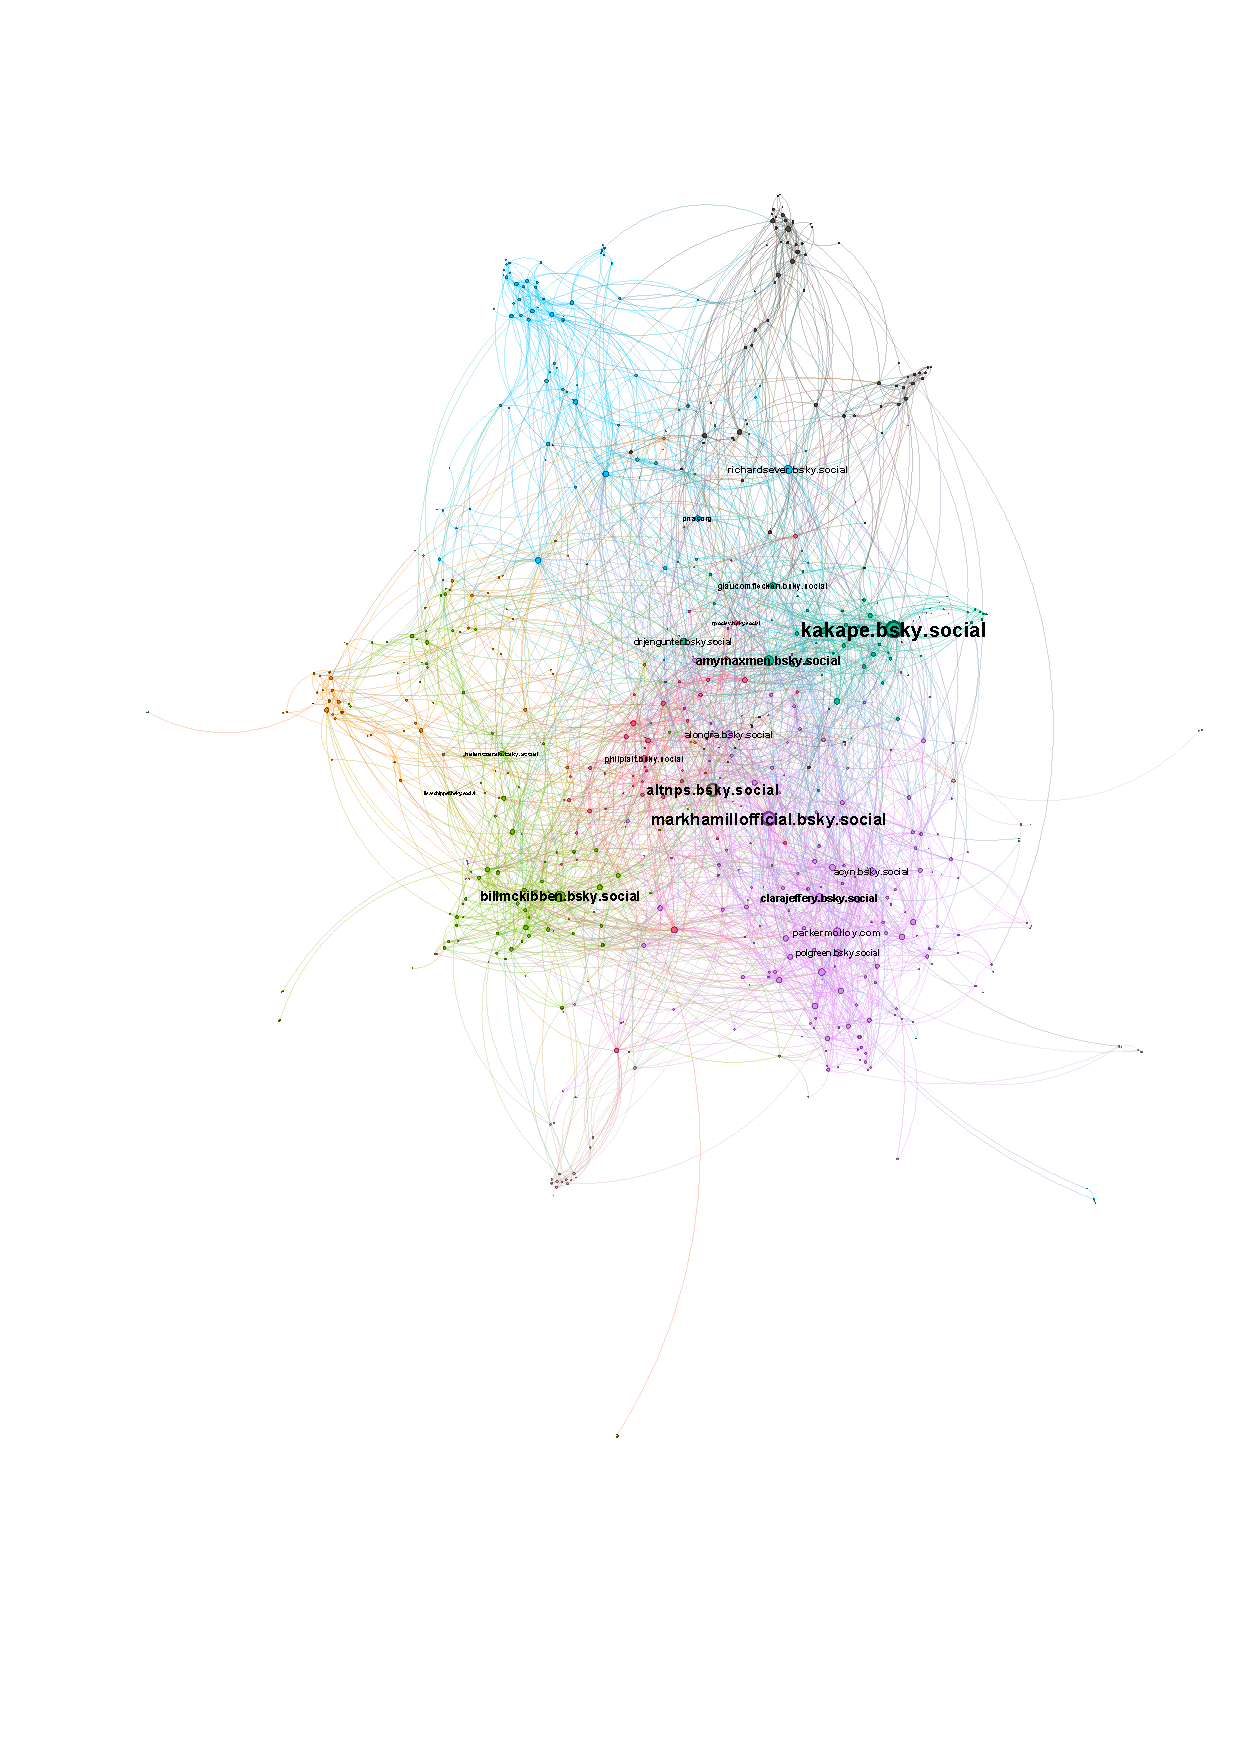
\includegraphics[width=\linewidth]{figures/network_communities.pdf}
  \caption{Bluesky scientific community: follow network (sampled subnetwork, ForceAtlas2 layout) colored by Louvain community and sized by degree.}
  \label{fig:communities}
\end{figure}

\subsection{Communities and the migration waves}
Combining the community labels with the account-creation dates (Section~\ref{sec:data}) shows that the two adoption waves of Figure~\ref{fig:creation} carry different disciplinary mixes (Figure~\ref{fig:cohorts}). The 2023 founding cohort is dominated by politics/news ($31\%$), followed by neuroscience ($15\%$) and climate/energy ($14\%$). The November-2024 migration cohort, the post-election exodus from X, is markedly more scientific: chemistry/biology more than doubles its share ($10\%\to20\%$) and conservation/ecology grows, while politics/news ($31\%\to24\%$), neuroscience and space recede. The later wave therefore did not amplify the political core but diversified the platform toward the natural sciences, a non-obvious effect that the static network alone would not reveal.

\begin{figure}[h]
  \centering
  
\includegraphics[width=\linewidth]{figures/cohort_composition.png}
  \caption{Disciplinary (Louvain-community) composition of the two adoption waves: the 2023 founding cohort vs the November-2024 migration cohort.}
  \label{fig:cohorts}
\end{figure}
